% Dissertation-ready template: Method of Manufactured Solutions (MMS)
% This file intentionally contains no report prose. Replace bracketed prompts
% and comment blocks with evidence drawn from the stored result directories.
\documentclass[11pt,a4paper]{article}

\usepackage[margin=28mm]{geometry}
\usepackage{amsmath,amssymb,bm}
\usepackage{booktabs,threeparttable}
\usepackage{graphicx}
\usepackage{siunitx}
\usepackage{hyperref}
\usepackage{cleveref}
\usepackage{xcolor}

\graphicspath{{./}{solns/}}
\newcommand{\placeholderfigure}[2]{%
  \fbox{\parbox[c][#2][c]{0.92\linewidth}{\centering\textit{Figure placeholder}\\[0.5em]#1}}%
}
\newcommand{\norm}[1]{\left\lVert #1 \right\rVert}
\newcommand{\seminorm}[1]{\left\lvert #1 \right\rvert}

\title{Verification of a Two-Dimensional Conjugate Heat-Transfer Solver\\
       by the Method of Manufactured Solutions}
\author{[Name]}
\date{[Month Year]}

\begin{document}
\maketitle

\begin{abstract}
% 150--220 words. State the verification objective, equations verified,
% discretisation range, the principal flow result, temperature-verification
% status, and one precise limitation. Do not explain the entire methodology.
\end{abstract}

\section{Introduction and verification scope}
% Target: 0.5--1 page.
% Explain why code verification is needed before interpreting physical CHT
% simulations. Define MMS as verification of the implemented equations and
% discretisation, not validation against experiment. State the scope exactly:
% 2D, steady, unit-square, smooth solution, global refinement, fluid domain.
% Explicitly exclude unverified claims: physical-model validity, transient
% behaviour, 3D, and fluid--solid MMS unless supporting results are added.

\section{Mathematical model and discretisation}
% Target: 1--1.5 pages. Use the notation actually used by the solver.
\subsection{Governing equations}
% Give the steady incompressible Navier--Stokes equations and the steady
% advection--diffusion temperature equation. Define u, p, T, nu, kappa, f, s.
\begin{align}
  (\bm{u}\cdot\nabla)\bm{u}-\nu\Delta\bm{u}+\nabla p &= \bm{f},
  & \nabla\cdot\bm{u} &= 0, \\
  \bm{u}\cdot\nabla T-\kappa\Delta T &= s.
\end{align}

\subsection{Finite-element approximation and error norms}
% State the Taylor--Hood pair precisely. In the present code, ``degree k''
% corresponds to Q_{k+1}/Q_k for velocity/pressure; verify and state the
% temperature polynomial space from the implementation before finalising.
% Define L2(u), L2(p), H1(u), and L2(T). Mention global mesh refinement,
% five refinement levels, and the pressure mean-value adjustment.
% Give expected asymptotic rates only after checking the exact FE spaces.

\section{Manufactured problem}
% Target: 1.5--2 pages. The exact expressions and source terms are generated
% from scripts/expressions_mms.py. Regenerate mms_report.tex if expressions
% change; include the generated equations rather than retyping them manually.
\subsection{Exact fields, forcing, and boundary data}
\begin{align}
  u_x &= \sin(\pi x)\cos(\pi y), &
  u_y &= -\cos(\pi x)\sin(\pi y), \\
  p &= \cos(\pi x)\sin(\pi y), &
  T &= \cos(2\pi x)\sin(\pi y).
\end{align}
% Insert the complete generated momentum and temperature source terms here,
% or move their long forms to an appendix and cite it. State that the velocity
% is divergence-free and that Dirichlet data are exact traces of these fields.

\begin{figure}[htbp]
  \centering
  % Replace this placeholder with:
  % 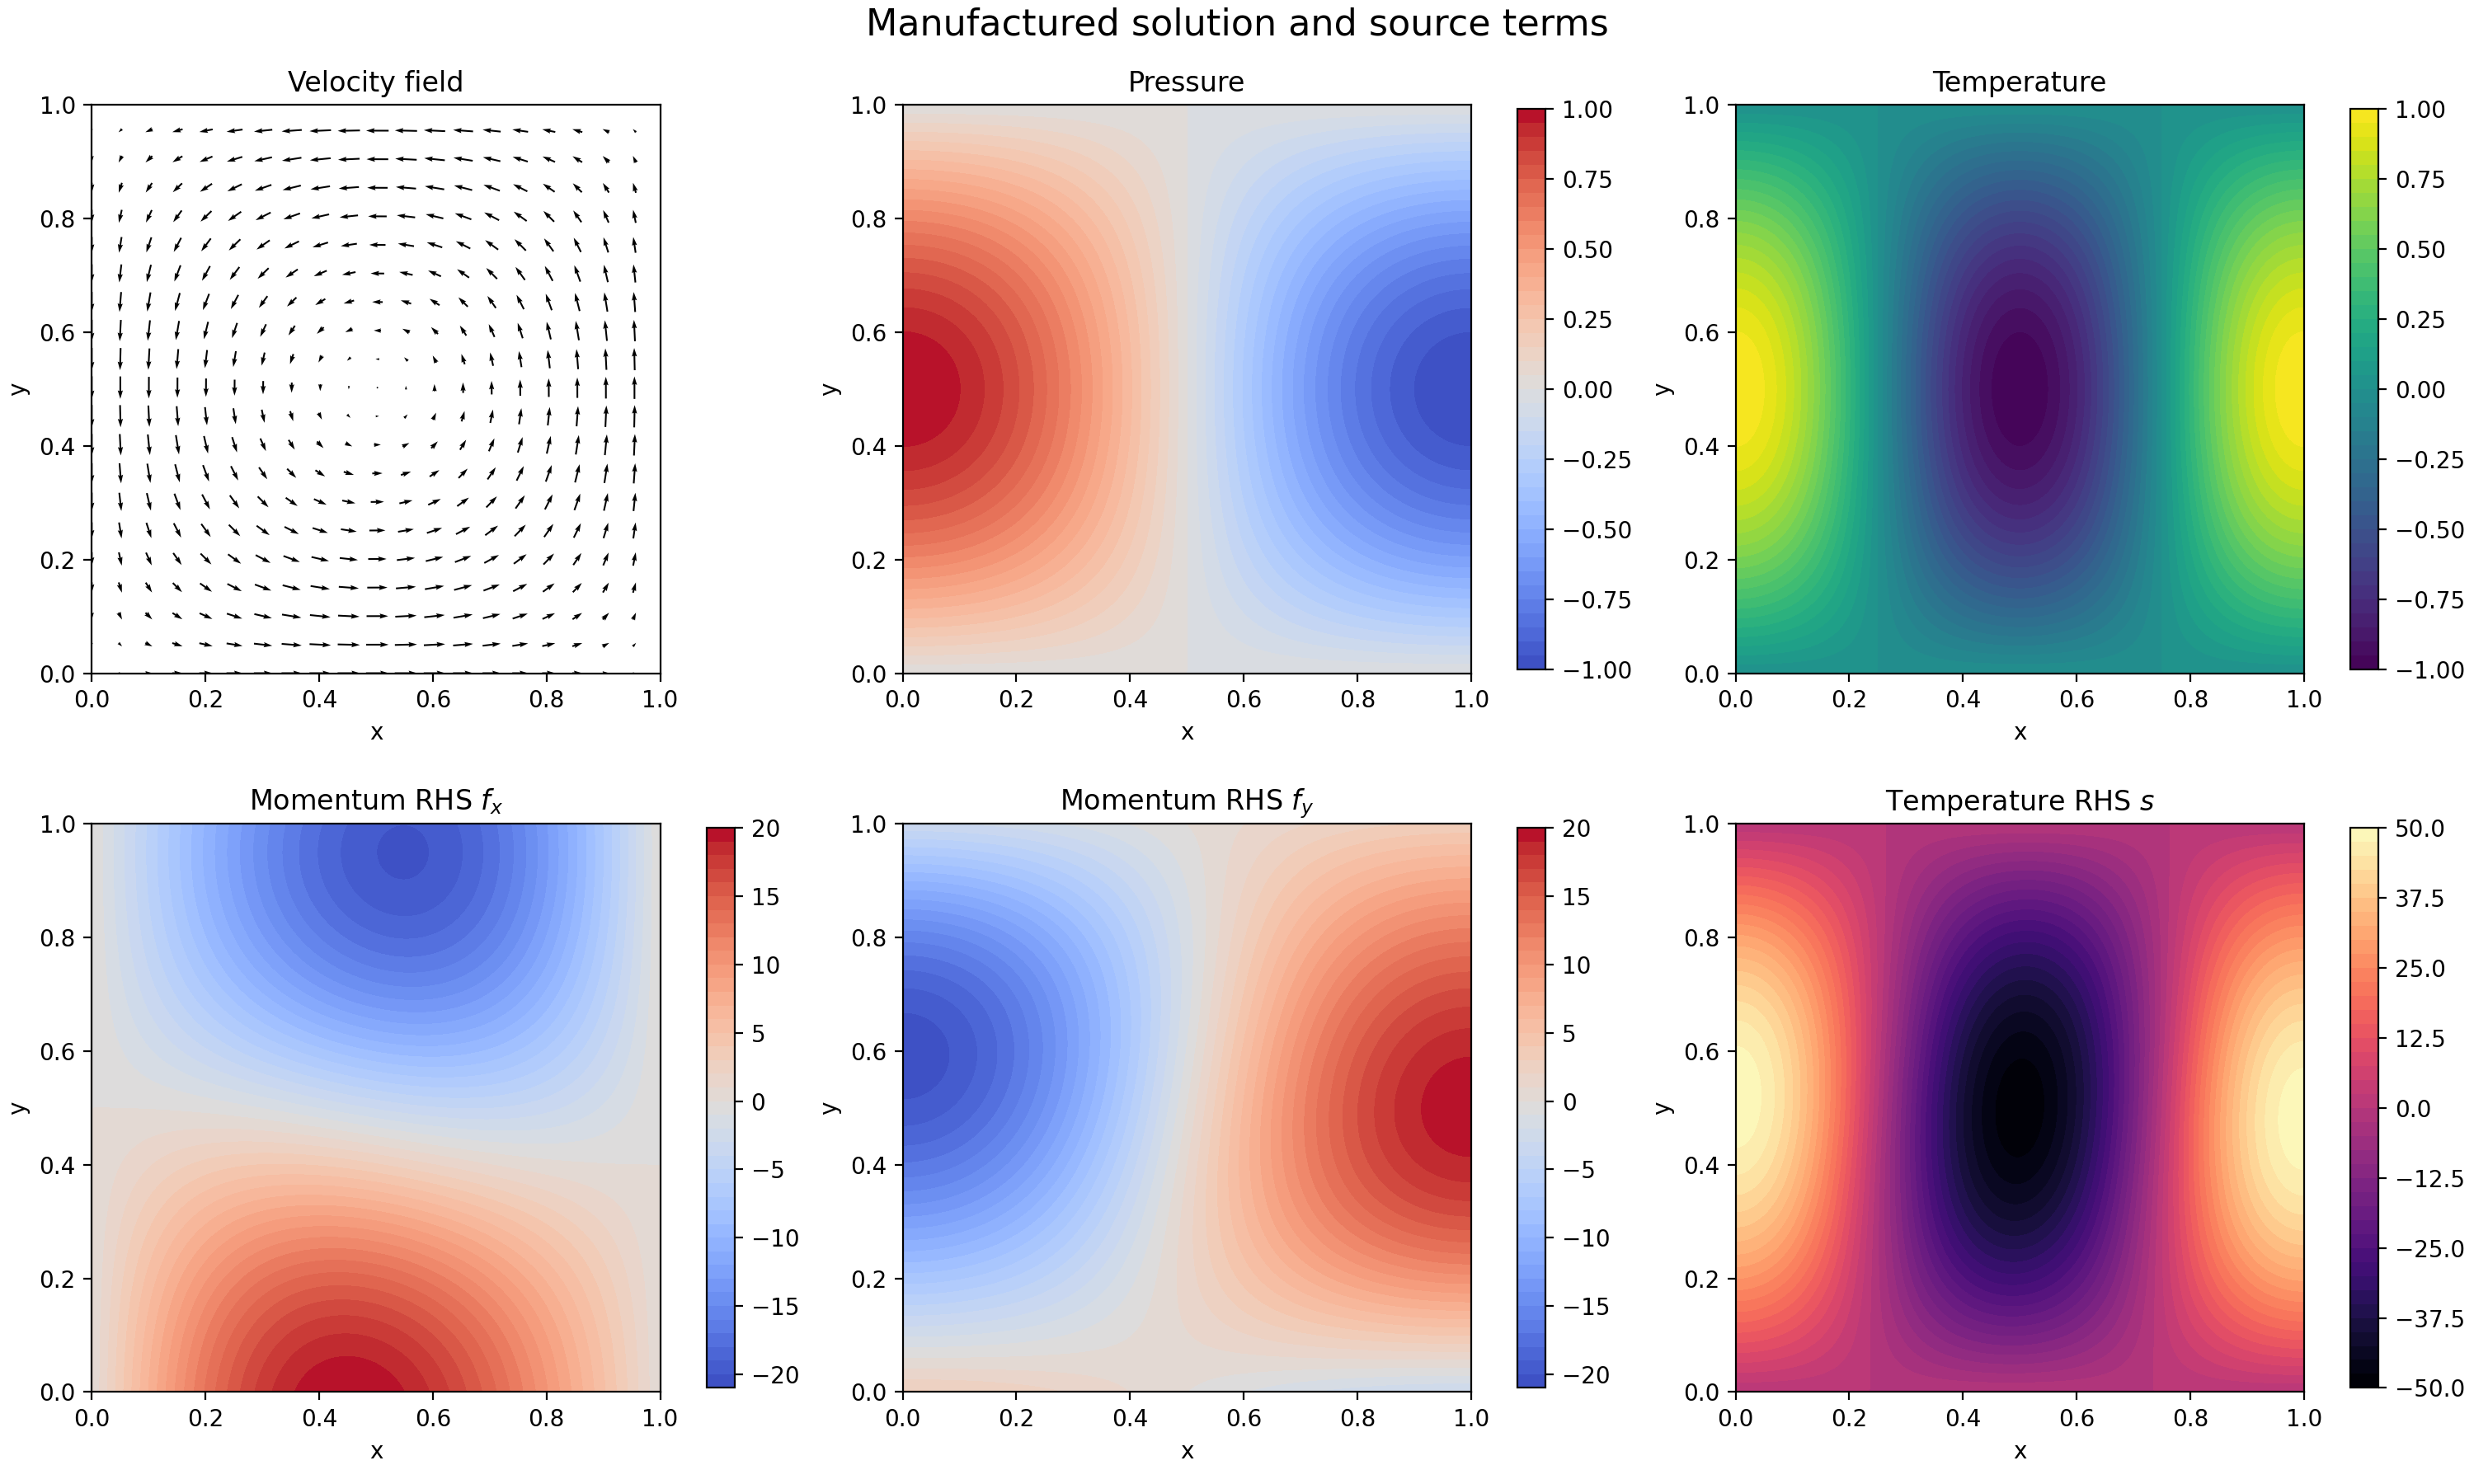
\includegraphics[width=\linewidth]{mms_visualization.png}
  \placeholderfigure{Exact velocity, pressure, temperature, and source terms.}{58mm}
  \caption{[Caption: identify each field and the parameters used to evaluate
  the forcing terms.]}
  \label{fig:mms-fields}
\end{figure}

\section{Computational verification procedure}
% Target: 1--1.5 pages.
% Report: square and square_finer meshes, Re=100 and Re=7500, degrees 1--3,
% number of refinement cycles, thermal diffusivity, nonlinear stopping rule,
% quadrature order, and how the fitted slopes are obtained. Include a short
% reproducibility paragraph: case files, output directory convention, and
% the script used for fitting. Do not report a fit that contains a numerical
% error floor without identifying/excluding those points.

\begin{table}[htbp]
  \centering
  \caption{Verification matrix and data availability.}
  \label{tab:verification-matrix}
  \begin{tabular}{ccccc}
    \toprule
    $Re$ & degree & flow norms & temperature $L^2$ & status \\
    \midrule
    100  & 1 & [yes] & [yes] & [analysed] \\
    100  & 2 & [yes] & [yes] & [floor assessment needed] \\
    100  & 3 & [yes] & [yes] & [floor assessment needed] \\
    7500 & 1 & [yes] & [not available] & [flow only] \\
    7500 & 2 & [yes] & [not available] & [flow only] \\
    7500 & 3 & [yes] & [not available] & [flow only] \\
    \bottomrule
  \end{tabular}
\end{table}

\section{Flow verification results}
% Target: 3--4 pages. This is the principal completed result.
% First give expected rates, then measured rates with standard errors. Discuss
% Re=100 and Re=7500 separately. Do not claim agreement merely because a
% rounded value is close: discuss uncertainty, local rates, and asymptotic
% range. Explicitly discuss the degree-1 H1 result at Re=7500.

\begin{table}[htbp]
  \centering
  \caption{Expected and fitted flow convergence rates.}
  \label{tab:flow-rates}
  \begin{threeparttable}
  \begin{tabular}{ccccc}
    \toprule
    $Re$ & degree & norm & expected rate & fitted rate \\
    \midrule
    [100/7500] & [1] & $\norm{\bm{u}-\bm{u}_h}_{L^2}$ & [ ] & [ ] \\
    [100/7500] & [1] & $\norm{p-p_h}_{L^2}$            & [ ] & [ ] \\
    [100/7500] & [1] & $\seminorm{\bm{u}-\bm{u}_h}_{H^1}$ & [ ] & [ ] \\
    % Add rows for degrees 2 and 3, or make separate tables by Reynolds number.
    \bottomrule
  \end{tabular}
  \begin{tablenotes}[flushleft]
    \footnotesize
    \item Fitted rates are slopes of least-squares fits in log--log space;
    report the standard error and state the refinement levels included.
  \end{tablenotes}
  \end{threeparttable}
\end{table}

\begin{figure}[htbp]
  \centering
  % Suggested source figures: error-global-q*_L2_velocity.png,
  % error-global-q*_L2_pressure.png, error-global-q*_H1_velocity.png.
  % Prefer a clean 1x3 composite for one degree or one 3x3 composite across
  % degrees; use consistent axes and identify Re in the caption.
  \placeholderfigure{Log--log flow-error convergence plots.}{65mm}
  \caption{[Caption: norms, Reynolds number, polynomial degrees, fit range,
  and whether all refinement levels are included.]}
  \label{fig:flow-convergence}
\end{figure}

\section{Coupled temperature verification}
% Target: 1.5--2 pages. Describe the added thermal source term, MMS thermal
% Dirichlet conditions, temperature error integration, and solver tolerance.
% At Re=100 there are results for degrees 1--3. Degree 1 gives a stable rate;
% degree 2 and 3 temperature errors become floor-dominated on fine meshes.
% Therefore report raw errors and local rates, but fit only defensible points
% or label full-range fits as non-asymptotic diagnostics. There are presently
% no corresponding coupled temperature runs at Re=7500.

\begin{table}[htbp]
  \centering
  \caption{Temperature $L^2$ errors and local convergence rates at $Re=100$.}
  \label{tab:temperature-rates}
  \begin{tabular}{cccccc}
    \toprule
    degree & cycle & cells & $\norm{T-T_h}_{L^2}$ & local rate & use in fit? \\
    \midrule
    [ ] & [ ] & [ ] & [ ] & [ ] & [yes/no, with reason] \\
    % Copy values from the selected final temperature-tightened result set.
    \bottomrule
  \end{tabular}
\end{table}

\begin{figure}[htbp]
  \centering
  % Suggested source figures: error-global-q*_L2_temperature.png from the
  % *_temperature_tighter directories. Make one composite plot if needed.
  \placeholderfigure{Temperature convergence plot, with floor-dominated
  refinement levels visibly distinguished.}{58mm}
  \caption{[Caption: state the fit range and explain any excluded points.]}
  \label{fig:temperature-convergence}
\end{figure}

\section{Spatial error diagnostics}
% Target: 0.75--1.5 pages. Explain that per-cell integrated errors diagnose
% spatial localisation and implementation problems; they are not a replacement
% for global convergence rates. Discuss only patterns visible in the figure.
% Use the final, consistent data set and specify Re, degree, and refinement.

\begin{figure}[htbp]
  \centering
  % Start from mms_integral_errors.png, but crop/rebuild a publication-sized
  % subset rather than inserting its entire dense 3x4 layout.
  \placeholderfigure{Selected per-cell velocity L2, velocity H1, and pressure
  L2 error fields.}{62mm}
  \caption{[Caption: identify the result set and explain colour-bar scaling.]}
  \label{fig:cell-errors}
\end{figure}

\section{Limitations and remaining verification work}
% Target: 0.75--1 page. Be explicit and constructive.
% Required: (i) thermal convergence at Re=7500 is missing; (ii) degree-2/3
% thermal fine-mesh results need a floor-aware analysis or reruns with a
% demonstrated tolerance criterion; (iii) the MMS is 2D/smooth/fluid-only;
% (iv) a separate manufactured fluid--solid problem would be required to claim
% verification of conjugate interface coupling.

\section{Conclusions}
% Target: 0.4--0.7 page. Give 3--5 numbered conclusions answering: what has
% been implemented, which flow claims are supported, what is supported for
% temperature, and the next experiment needed to close the verification matrix.

\appendix
\section{Generated MMS forcing terms and boundary values}
% Paste or \input the generated mms_report.tex material here after checking
% it matches the code version used to produce the reported results.

\section{Complete convergence tables}
% Include the generated convergence_rates.tex tables for every reported set.
% Put exploratory/obsolete directories in a separate archival appendix or omit
% them. Record the exact result-directory names for reproducibility.

\end{document}
